
\section{����}
\label{sec:heart_discussion}

The computer programs implemented for this work were written in C++.
As a matter of fact, one of the keys in the proposed approach is the well-chosen thresholds in the binary thresholding step before the computation of initial contours and edge potential maps. %
In the results of this step, most of the irrelevant contents (i.e., aorta, pericardium, etc.) were successfully excluded otherwise can inevitably affect the following computation.
In the evolution phase, the locations of the seeding points were vital, especially for those located at the vicinities of the indistinct boundaries between the heart and its surrounding organs. %
To visualize the surface model, the iso-surface information were extracted and rearranged by the marching cubes method \cite{Lorensen1987MC}.
Considering the context of this work, only an approximating surface model of the heart was delineated, which was sufficient for the intuition purpose (see Fig. \ref{fig:heart_overlay}).
\begin{figure}[t]
\centering
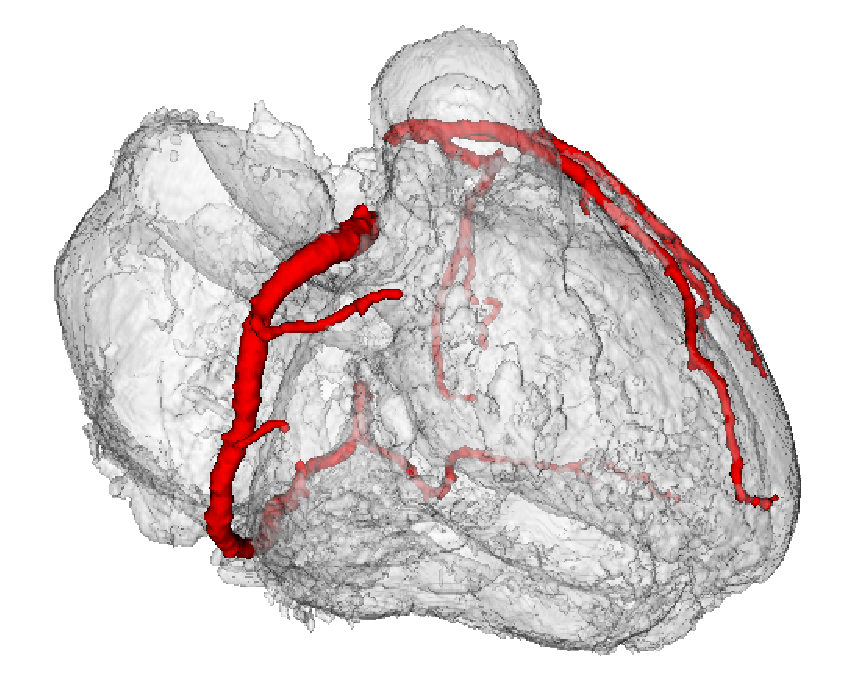
\includegraphics[height=2.4in]{figures/heart/heart_with_ca.eps}
%\caption{The overlayed three-dimensional models of the heart and the coronary arteries acquired in the previous work \cite{Yang2013ROBIO} are rendered in the same scene.}
\caption{The overlayed three-dimensional models of the heart and the coronary arteries are rendered in the same scene.}
\label{fig:heart_overlay}
\end{figure} 